\section{The LBM in brief}

\subsection*{Linearized Boltzmann equation}

Here we want to repeat a few very basic facts about the LBM. 
You will find much better introductions in various books and
articles, e.g. \cite{succi01a, duenweg09a}. It will however help clarifying 
our choice of words and we will eventually say something about the 
implementation in \ES{}. It is very loosely written, with the goal that
the reader understands basic concepts and how they are implemented in \ES{}.


The LBM essentially consists of solving a fully discretized
version of the linearized Boltzmann equation. The Boltzmann equation
describes the time evolution of the one particle distribution
function $f\left(x,p,t\right)$, which is the probability to find a molecule in a phase
space volume $\d x \d p$ at time $t$.The function $f$ is normalized
so that the integral over the whole phase space is the total 
mass of the particles:
\begin{equation*}
  \int f\left(x,p\right)\d x \d p = Nm,
\end{equation*}
where $N$ denotes the particle number and $m$ the particle mass.
The quantity f$\left(x,p\right)\d x \d p$ corresponds
to the mass of particles in this particular cell of the phase
space, the population. \\

\subsection*{Discretization}
The LBM discretizes the Boltzmann equation not only in real
space (the lattice!) and time, but also the velocity space is discretized.
A surprisingly small number of velocities, in 3D usually 
19, is sufficient to describe incompressible, viscous flow correctly.
Mostly we will refer to the three-dimensional model with a discrete
set of 19 velocities, which is conventionally called D3Q19.
These velocities, $\vec c_i$,
are chosen so that they correspond to the movement from one lattice
node to another in one time step. A two step scheme is used to transport
information through the system: In the streaming step
the particles (in terms of populations) are transported
to the cell where they corresponding velocity points to. 
In the collision step, the distribution functions
in each cell are relaxed towards the local thermodynamic
equilibrium. This will be described in more detail below.

\begin{figure}[htp]
\begin{center}
  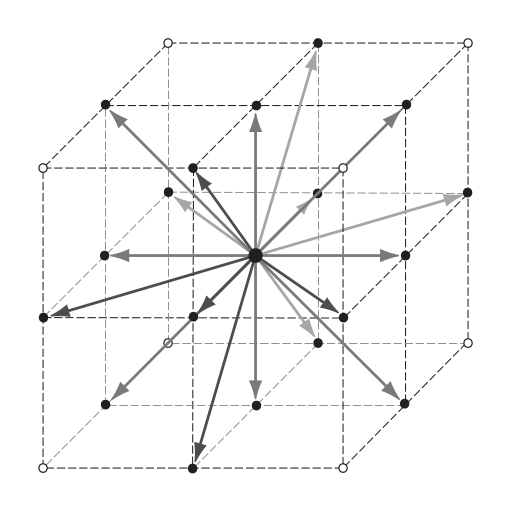
\includegraphics[height=0.3\textheight]{figures/latticeboltzmann-grid}
  \caption[]{The 19 velocity vectors $\vec{c}_{i}$ for a D$3$Q$19$ lattice. From
  the central grid point, the velocity vectors point towards all 18
  nearest neighbours marked by filled circles. The 19th velocity vector is the
  rest mode (zero velocity).}
  \label{fig:model-d3q18grid}
\end{center}
\end{figure}

The hydrodynamic fields, the density, 
the fluid momentum density,
the pressure tensor can be calculated straightforwardly from
the populations: They correspond to the moments
of the distribution function: 
\begin{align}
  \rho &= \sum f_i \\
  \vec{j} = \rho \vec{u} &= \sum f_i \vec{c_i} \\
  \Pi^{\alpha \beta} &= \sum f_i \vec{c_i}^{\alpha}\vec{c_i}^{\beta} 
  \label{eq:fields}
\end{align}
Here the Greek indices denotes the cartesian axis and the
Latin indices indicate the number in the disrete velocity set.
Note that the pressure tensor is symmetric.
It is easy to see that these equations are linear transformations
of the $f_i$ and that they carry the most important information. They
are 10 independent variables, but this is not enough to store the
full information of 19 populations. Therefore 9 additional quantities
are introduced. Together they form a different basis set of the
19-dimensional population space, the modes space and the modes are denoted by 
$m_i$. The 9 extra modes are referred to as kinetic modes or
ghost modes. It is possible to explicitly write down the 
base transformation matrix, and its inverse and in the \ES{}
LBM implementation this basis transformation is made for every
cell in every LBM step. It is possible to write a code that does not
need this basis transformation, but it has been shown, that this
only costs 20\% of the computational time and allows for 
larger flexibility.

\subsection*{The second step: collision}
The second step is the collision part, where
the actual physics happens. For the LBM it is assumed that
the collision process linearly relaxes the populations to the local
equilibrium, thus that it is a linear (=matrix) operator 
acting on the populations in each LB cell. It should conserve 
the particle number and the momentum. At this point it is clear
why the mode space is helpful. A 19 dimensional matrix that
conserves the first 4 modes (with the eigenvalue 1) is diagonal in the
first four rows and columns.
Some struggling with lattice symmetries shows that four independent
variables are anough to characterize the linear relaxation
process so that all symmetries of the lattice are obeyed. 
Two of them are closely related to 
the shear and bulk viscosity of the fluid, and two of them
do not have a direct physical equivalent. They are just called
relaxation rates of the kinetic modes.


The equilibrium distribution to which the populations relax 
is obtained from maximizing the information entropy 
$\sum f_i \log f_i$ under the constraint that the density
and velocity take their particular instantaneous 
values. 

In mode space the equilbrium distribution is calculated much from 
the local density and velocity.
The kinetic modes 11-19 have the value 0 in equilibrium.
The collision operator is diagonal in mode space
and has the form
\begin{align*}
  m^\star_i &= \gamma_i \left( m_i - m_i^\text{eq} \right) + m_i ^\text{eq}.
\end{align*}
Here $m^\star_i$ is the $i$th mode after the collision.
In words we would say: Each mode is relaxed towards
it's equilibrium value with a relaxation rate $\gamma_i$.
The conserved modes are not relaxed, or, the corresponding
relaxation parameter is one.

By symmetry consideration one finds that only four independent
relaxation rates are allowed. We summarize them here.
\begin{align*}
  m^\star_i &= \gamma_i m_i  \\
  \gamma_1=\dots=\gamma_4&=1 \\
  \gamma_5&=\gamma_\text{b} \\
  \gamma_6=\dots=\gamma_{10}&=\gamma_\text{s} \\
  \gamma_{11}=\dots=\gamma_{16}&=\gamma_\text{odd} \\
  \gamma_{17}=\dots = \gamma_{19}&=\gamma_\text{even} \\
\end{align*}

To include hydrodynamic fluctuations of the fluid, 
random fluctuations are added to the nonconserved modes $4\dots 19$ on every LB node so that
the LB fluid temperature is well defined and the corresponding
fluctuation formula, according to the fluctuation dissipation theorem holds.
An extensive discussion of this topic is found in \cite{duenweg07a}

\subsection*{Particle coupling}

Particles are coupled to the LB fluid with the force coupling:
The fluid velocity at the position of a particle is calculated 
by a multilinear interpolation and a force is applied on the particle
that is proportional to the velocity difference between particle 
and fluid:
\begin{equation}
  \vec{F}_D = - \gamma \left(v-u\right) 
  \label{eq:model-lbcoupling}
\end{equation}
The opposite force is distributed on the surrounding LB nodes. Additionally
a random force is added to maintain a constant temperature, according
to the fluctuation dissipation theorem. 
\begin{figure}[htp]
\begin{center}
   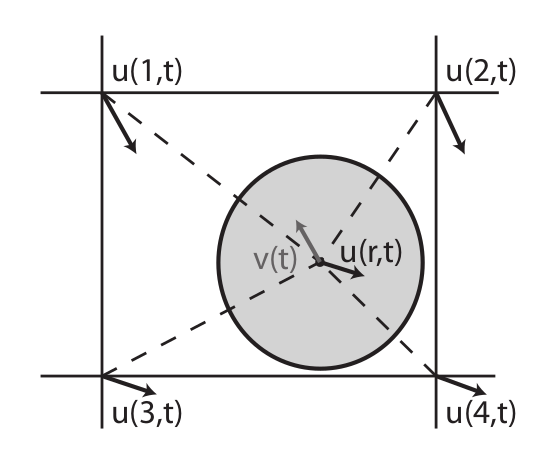
\includegraphics[height=0.3\textheight]{figures/latticeboltzmann-momentumexchange}
   \caption{The coupling scheme between fluid and particles is based on the
   interpolation of the fluid velocity $\vec{u}$ from the grid nodes.  
   This is done by linear interpolation. The difference between the
   actual particle velocity $\vec{v}(t)$ and the interpolated velocity
   $\vec{u}(\vec{r},t)$ is used in the momentum exchange of
   Equation~\ref{eq:model-lbcoupling}.}
  \label{fig:model-lbcoupling}
\end{center}
\end{figure}
\pagebreak
